% !TeX program = pdflatex
\documentclass[tikz,border=8pt]{standalone}
\usepackage{tikz}
\definecolor{FigureBlue}{HTML}{2563EB}\definecolor{FigureOrange}{HTML}{EA580C}
\begin{document}
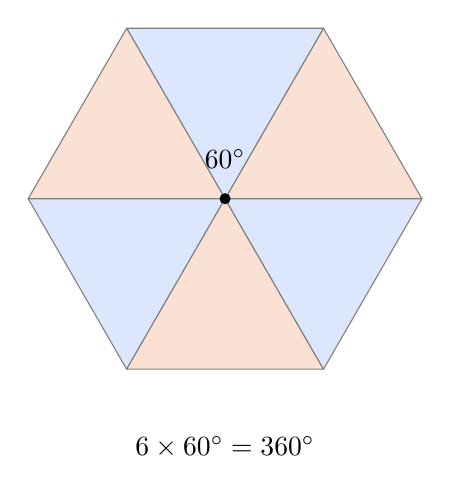
\begin{tikzpicture}[line join=round]
  \foreach \k in {0,...,5}{\pgfmathsetmacro{\a}{60*\k}\pgfmathsetmacro{\b}{60*(\k+1)}\pgfmathtruncatemacro{\shade}{mod(\k,2)}\ifnum\shade=0\def\tilecolor{FigureOrange!18}\else\def\tilecolor{FigureBlue!16}\fi\fill[fill=\tilecolor,draw=gray] (0,0)--(\a:2.5)--(\b:2.5)--cycle;}
  \fill (0,0) circle (2pt); \node at (0,0.5) {$60^\circ$};
  \node at (0,-3.15) {$6\times60^\circ=360^\circ$};
\end{tikzpicture}
\end{document}
